%% The first command in your LaTeX source must be the \documentclass command.
%%
\documentclass[etq]{acnsart}

\setdoi{10.55056/etq.1126}
\setjournalyear{2026}
%\setjournalvolume{2026}
%\setjournalissue{2}
\setcounter{page}{1}

\usepackage{enumitem}
\usepackage{tikz, pgfplots, pgf-pie, longtable, tabularx, makecell, booktabs, multirow}
\pgfplotsset{compat=1.18}
\usetikzlibrary{shapes, arrows, positioning, chains}
\usepackage{xcolor}
\usepackage{amsmath}

\begin{document}
	
	%\let\WriteBookmarks\relax
	%\def\floatpagepagefraction{1}
	%\def\textpagefraction{.001}
	%
	%\shorttitle{Methodological quality in gamification research for history education}
	
	\title{Methodological quality and reporting practices in~gamification research for history education: a~critical methodological analysis}
	
	%\shortauthors{S. S. Korniienko and S. O. Semerikov}
	
	\author[1]{Serhii S. Korniienko}[%
	orcid={0000-0002-2573-2115},
	email={korniienko.serhii@kdpu.edu.ua}
	]
	
	\author[1,2,3,4]{Serhiy O. Semerikov}[
	orcid=0000-0003-0789-0272,
	email={semerikov@gmail.com},
	url={https://acnsci.org/semerikov}
	]
	
	
	%\cortext[cor1]{Corresponding author}
	
	\address[1]{Kryvyi Rih State Pedagogical University, 54 Universytetskyi Ave., Kryvyi Rih, 50086, Ukraine}
	\address[2]{Academy of Cognitive and Natural Sciences, 54 Universytetskyi Ave., Kryvyi Rih, 50086, Ukraine}
	\address[3]{Institute for Digitalisation of Education of the NAES of Ukraine, 9 M. Berlynskoho Str., Kyiv, 04060, Ukraine}
	\address[4]{Zhytomyr Polytechnic State University, 103 Chudnivsyka Str., Zhytomyr, 10005, Ukraine}
	
	
	% ===========================================================================
	% REVISED ABSTRACT
	% ===========================================================================
	
	\begin{abstract}
		Gamification has attracted growing research attention as an instructional strategy for history education, yet the methodological rigour of this evidence base has not been systematically evaluated. This study presents a secondary methodological analysis of 74 empirical studies included in a recent systematic review of gamification in history education \cite{KorniienkoSemerikov2024}, published between 2004 and 2024 across 27 countries. We introduce a ten-item Methodological Reporting Quality Score (MRQS) to assess the completeness and rigour of reporting practices, and we re-analyse risk-of-bias assessments across three adapted ROBIS domains. The mean MRQS was 4.31 out of 10 (SD = 1.93, median = 4.0), indicating substantial gaps in methodological reporting. The most frequently satisfied criteria were the presence of a theoretical framework (94.6\%) and explicit reporting of sample size (83.8\%), while the least satisfied were reporting of effect sizes (9.5\%), provision of an explicit definition of gamification or game-based learning (14.9\%), and use of validated measurement instruments (21.6\%). Risk-of-bias analysis confirmed that 83.8\% of studies received a high overall rating, with Domain~1 (sampling and selection, 85.1\% high) representing the most persistent source of weakness~-- no study received a favourable rating on sample representativeness~-- followed by Domain~2 (data collection and analysis, 63.5\% high) and Domain~3 (interpretation and reporting, 55.4\% high). Studies providing explicit gamification definitions scored higher on the MRQS (5.36 vs.\ 4.13, \textit{p} = .065) but showed equivalent risk-of-bias ratings, suggesting that definitional clarity functions as a marker of reporting conscientiousness rather than of design rigour. Comparison of GPT-4o's automated risk-of-bias assessments against human-verified judgments revealed only 37.6\% overall agreement (Cohen's $\kappa$ = --0.04 to 0.21), with the model consistently applying less stringent criteria than human reviewers, while factual metadata extraction across multiple LLMs achieved 82--97\% pairwise agreement. These findings indicate that the current evidence base for gamification in history education suffers from pervasive methodological shortcomings that limit the strength of causal inferences and preclude meta-analytic synthesis. We propose the MRQS as a replicable, domain-adapted instrument for assessing reporting quality in educational technology research.
	\end{abstract}
	
	%\begin{highlights}
	%	\item Methodological Reporting Quality Score (MRQS) applied to 74 gamification-in-history studies.
	%	\item Mean MRQS was 4.31/10; only 9.5\% reported effect sizes and 21.6\% used validated instruments.
	%	\item 83.8\% of studies exhibited high overall risk of bias; 0\% met sample representativeness criteria.
	%	\item Definitional clarity is associated with better reporting but not with stronger study design.
	%	\item LLM risk-of-bias assessment showed near-chance agreement ($\kappa \leq 0.21$) with human verification.
	%\end{highlights}
	
	
	\begin{keywords}
		gamification \sep history education \sep methodological quality \sep risk of bias \sep reporting practices \sep systematic review
	\end{keywords}
	
	\maketitle
	
	
	% ===========================================================================
	% SECTION 1: INTRODUCTION
	% ===========================================================================
	
	\section{Introduction}
	\label{sec:introduction}
	
	\subsection{Background}
	\label{sec:intro_background}
	
	The application of game design elements in educational contexts has attracted substantial scholarly attention over the past two decades. Since \citet{Deterding2011} proposed the widely adopted definition of gamification as ``the use of game design elements in non-game contexts'' \cite[p.~9]{Deterding2011}, research on gamified and game-based approaches to learning has expanded rapidly across disciplines, education levels, and geographic settings. Systematic reviews and meta-analyses have documented generally positive effects of gamification on learner motivation, engagement, and knowledge acquisition \cite{Hamari2014, Sailer2017, Connolly2012}, though with important caveats regarding heterogeneity in effects and the conditions under which these approaches are most effective \cite{Clark2016, DichevDicheva2017}.
	
	Within this broader research programme, history education represents a distinctive application domain. Unlike STEM disciplines, where learning outcomes can often be measured through standardised assessments of procedural or factual knowledge, history education foregrounds interpretive reasoning, perspective-taking, source evaluation, and narrative construction~-- competencies that resist straightforward quantification \cite{12Gilbert2019108, 46Stirling2022}. Gamified approaches in history have consequently spanned a wide range of formats, from commercial strategy titles such as \textit{Civilization~IV} \cite{55Squire2004} and narrative-driven games such as \textit{Assassin's Creed} \cite{12Gilbert2019108}, to custom-designed virtual reality reconstructions of archaeological sites \cite{1Barbatsis201159}, location-based augmented reality games \cite{51Ardito2007}, and physical board games designed around historical role-play \cite{38Mercik2024}. This diversity of interventions, coupled with the discipline's interpretive demands, makes the evidence base for gamification in history education both rich and methodologically heterogeneous.
	
	A recent systematic review by \citet{KorniienkoSemerikov2024} synthesised 74 empirical studies on gamification in history education published between 2004 and 2024, drawn from Scopus, Web of Science, and Dimensions. That review documented predominantly positive findings for knowledge acquisition and student engagement, but also identified pervasive methodological limitations: 83.8\% of studies received a high overall risk-of-bias rating, 85.1\% provided no explicit definition of gamification, median sample sizes were small (approximately 34 participants), and only 31.1\% of studies included a control or comparison group. These figures suggest that the optimistic effectiveness narrative may rest on a methodologically fragile foundation.
	
	\subsection{The need for methodological scrutiny}
	\label{sec:intro_need}
	
	Systematic reviews in educational technology have traditionally focused on synthesising effectiveness findings~-- documenting whether an intervention ``works'' according to various outcome measures. Comparatively less attention has been given to the systematic appraisal of how that evidence is produced, reported, and interpreted. This imbalance matters because the strength of effectiveness claims depends entirely on the methodological rigour of the primary studies from which they are derived. When reviews conclude that gamification ``shows promise'' or ``enhances engagement'', the practical value of such conclusions hinges on whether the underlying studies employed adequate sample sizes, appropriate comparison conditions, validated measurement instruments, and transparent reporting of statistical results.
	
	Several lines of evidence suggest that methodological quality is a persistent concern in educational technology research generally, and in gamification research specifically. \citet{DichevDicheva2017} observed that gamification studies frequently lack control groups, use convenience samples, and rely on self-reported outcomes, raising questions about the internal and external validity of reported effects. \citet{KoivistoHamari2019}, reviewing motivational information systems research, noted a similar pattern of small sample sizes and limited use of validated instruments. \citet{Connolly2012}, in a large-scale review of serious games, found that a majority of included studies exhibited significant methodological limitations. In the specific domain of history education, \citet{Oceja2022419} observed that studies using games for teaching history frequently lacked formal empirical evaluation of their educational impact.
	
	These concerns are not merely academic. Methodological shortcomings introduce systematic biases that can inflate effect estimates, generate false-positive findings, and produce an evidence base that appears more conclusive than warranted. Small samples increase the likelihood of both Type~I and Type~II errors. The absence of control groups precludes causal inference. Unvalidated instruments may poorly or inconsistently measure constructs across studies. The failure to report effect sizes prevents meaningful cross-study comparison and meta-analytic synthesis. And the absence of explicit definitions creates conceptual ambiguity, undermining the very construct being investigated.
	
	Despite these recognised problems, no study has systematically quantified the methodological quality of the gamification-in-history-education literature using a structured assessment framework. Existing reviews, including the parent review by \citet{KorniienkoSemerikov2024}, assess risk of bias at the study level as part of the review methodology, but they do not treat methodological quality itself as the primary object of investigation. The result is that the field possesses a growing body of evidence about whether gamification is effective in history education, but lacks a structured account of how trustworthy that evidence actually is.
	
	\subsection{LLM-assisted research synthesis: a methodological opportunity}
	\label{sec:intro_llm}
	
	A related and increasingly consequential methodological question concerns the role of large language models (LLMs) in systematic review processes. The parent review by \citet{KorniienkoSemerikov2024} employed GPT-4o for data extraction and risk-of-bias assessment, with Claude~3.5~Sonnet used for initial eligibility screening. The use of LLMs in research synthesis is growing rapidly, driven by the promise of reduced time and labour costs, particularly for large-scale reviews. However, the reliability of LLM-generated assessments~-- especially for subjective judgements such as risk of bias~-- remains an open empirical question. Documenting the agreement between LLM assessments and human judgements, and identifying domains where automated assessment is more or less reliable, is necessary both for evaluating the trustworthiness of the parent review's findings and for informing best practices in AI-assisted research synthesis.
	
	\subsection{Objectives and research questions}
	\label{sec:intro_objectives}
	
	This paper undertakes a secondary methodological analysis of the 74 studies included in the systematic review by \citet{KorniienkoSemerikov2024}. Rather than re-examining the effectiveness of gamification in history education, we treat the methodological characteristics and reporting practices of the primary studies as the primary object of inquiry. Our aims are threefold: (1)~to characterise the prevailing research designs, measurement practices, and reporting conventions in this literature; (2)~to construct and apply a structured quality metric~-- the Methodological Reporting Quality Score (MRQS)~-- that enables systematic comparison across studies, time periods, and study-level characteristics; and (3)~to examine the reliability of LLM-assisted assessment in the context of this review.
	
	The following research questions guide this analysis:
	
	\begin{enumerate}[label=RQ\arabic*:,leftmargin=*]
		\item What are the prevailing methodological designs in gamification research for history education, and how do they distribute across time, geography, education level, and game type?
		\item What is the quality of measurement and reporting practices across included studies, as assessed by the Methodological Reporting Quality Score (MRQS)?
		\item What patterns of risk of bias emerge across the three adapted ROBIS domains, and what study-level characteristics are associated with higher or lower methodological quality?
		\item To what extent do conceptual and definitional practices (or their absence) correlate with methodological rigour?
		\item What is the reliability of using large language models (GPT-4o, Claude~3.5~Sonnet) for automated risk-of-bias assessment and data extraction in educational technology systematic reviews?
	\end{enumerate}
	
	\subsection{Scope and contribution}
	\label{sec:intro_contribution}
	
	This paper makes three principal contributions. First, the MRQS provides a replicable, domain-adapted instrument for assessing reporting quality in gamification research for history education. While not a substitute for full risk-of-bias assessment, the MRQS distils ten binary indicators of reporting completeness that can be reliably coded from published study reports, enabling both descriptive mapping and cross-tabulation with study-level variables.
	
	Second, the re-analysis of risk-of-bias data at the domain level (sampling, measurement, interpretation) offers a more granular account of where methodological weaknesses are concentrated than the overall ratings reported in the parent review. This domain-level decomposition identifies specific targets for methodological improvement.
	
	Third, documenting LLM agreement patterns contributes to the emerging evidence base on automated research synthesis tools, with implications for the growing number of systematic reviews that employ them.
	
	It is important to be clear about what this paper does \emph{not} do. We do not conduct new primary data collection; all analyses are based on data extracted and reported in \citet{KorniienkoSemerikov2024}. We do not re-extract data from the original study PDFs. We do not perform meta-analysis, as the heterogeneity of interventions and outcomes in this literature precludes meaningful statistical pooling. And we do not make normative claims about whether individual studies are ``good'' or ``bad''~-- the MRQS and risk-of-bias assessments describe reporting practices and study design features, not the intellectual merit or practical significance of the research.
	
	The remainder of this paper is structured as follows. Section~\ref{sec:methods} describes the data source, the construction of the MRQS, the risk-of-bias re-analysis procedure, the LLM validation protocol, and the statistical methods employed. Section~\ref{sec:results} presents findings organised by research question. Section~\ref{sec:discussion} discusses the implications of these findings for the gamification-in-history-education literature and for research practice in educational technology more broadly. Section~\ref{sec:conclusion} summarises conclusions and presents a proposed reporting checklist for future studies.
	
	
	% ===========================================================================
	% SECTION 2: METHODS
	% ===========================================================================
	
	\section{Methods}
	\label{sec:methods}
	
	This study is a secondary methodological analysis of data collected and reported in a prior systematic review. No new primary data were gathered; all analyses draw on the structured data files, risk-of-bias assessments, and study characteristics extracted in the parent review \cite{KorniienkoSemerikov2024}. The study did not involve human participants and therefore did not require ethical approval.
	
	\subsection{Data source}
	\label{sec:methods_datasource}
	
	The data for this analysis originate from a systematic review of gamification in history education \cite{KorniienkoSemerikov2024}, which followed the PRISMA 2020 statement \cite{Page2021}. That review searched Scopus, Web of Science, and Dimensions from inception to July~17, 2024, identifying an initial pool of 4,011 records. After deduplication, title--abstract screening, and full-text assessment, 80 studies advanced to data extraction. Of these, six were excluded during detailed analysis (three were not about history education, one was a systematic review rather than a primary study, one was about the history of mathematics, and one contained no gamification intervention), yielding 74 included studies published between 2004 and 2024 across 27 countries.
	
	For each included study, the parent review produced a structured data extraction record in JSON format conforming to a pre-specified schema. Each record contained: bibliographic metadata (authors, year, publication type, venue, DOI); study characteristics (country, education level, sample size, study design, game type, game name, study aim); eligibility judgments; data for each of the four review research questions (RQ1: definitions and theoretical frameworks; RQ2: effectiveness and outcomes; RQ3: game design and instructional strategies; RQ4: challenges and limitations); and a risk-of-bias assessment across three adapted ROBIS domains with six signalling questions, domain-level judgments, an overall rating, and supporting evidence extracts. These 74 JSON records, together with the tabulated risk-of-bias assessments, study characteristics tables, and aggregate statistics files, constitute the data corpus for the present analysis.
	
	\subsubsection{Data extraction in the parent review}
	
	Data extraction in the parent review was automated using the GPT-4o, a large language model, which received each study's PDF as input alongside a structured 21-item prompt covering all review research questions. One researcher subsequently verified the GPT-4o outputs. Eligibility screening was initially performed by Claude~3.5~Sonnet against seven binary criteria, with two researchers independently reviewing and resolving disagreements by consensus. Risk-of-bias assessment was likewise performed by GPT-4o using a structured prompt requesting yes/no/unclear responses to six signalling questions, with subsequent human verification. These automated-then-verified extraction procedures are relevant to the present analysis because the MRQS and risk-of-bias re-analysis both operate on the resulting data; any systematic biases introduced during LLM-assisted extraction would propagate into our findings.
	
	\subsection{Methodological Reporting Quality Score (MRQS)}
	\label{sec:methods_mrqs}
	
	To assess the completeness and rigour of reporting practices across the 74 included studies, we constructed a Methodological Reporting Quality Score (MRQS) comprising ten binary items (coded 0 or 1), yielding a composite score ranging from 0 to 10. The ten items were selected to capture fundamental aspects of methodological reporting that are widely endorsed in educational research guidelines \cite{Schulz2010CONSORT, HigginsThomas2019} and that are codable from the structured data extracted in the parent review without requiring re-access to original study PDFs.
	
	Table~\ref{tab:mrqs_items} presents the ten items, their rationale, and the specific data fields used for coding.
	
	\begin{table}[!ht]
		\centering
		\caption{Methodological Reporting Quality Score (MRQS): item definitions and coding rules.}
		\label{tab:mrqs_items}
		%\setlength\tabcolsep{3pt}
		%\small
		\resizebox{\linewidth}{!}{
			\begin{tabularx}{1.005\linewidth}{@{}c  p{0.18\textwidth} X p{0.38\textwidth}@{}}
				\toprule
				\textbf{Item} & \hfil \textbf{Criterion} & \hfil \textbf{Rationale} & \hfil \textbf{Data source and coding} \\
				\midrule
				M1 & Sample size explicitly reported & Transparent reporting of participant numbers is a minimum requirement for evaluating statistical conclusions & Coded 1 if \texttt{sample\_size} $\neq$ null in the study characteristics record \\
				\addlinespace
				M2 & Sample size $\geq$ 30 & A threshold of 30 participants is commonly regarded as the minimum for basic parametric inference and for the central limit theorem to provide reasonable approximations & Coded 1 if \texttt{sample\_size} $\geq 30$ \\
				\addlinespace
				M3 & Control or comparison group present & Comparison conditions are necessary for causal inference about intervention effects & Coded 1 if the study was identified in the parent review's verified list of 23 studies with control or comparison groups \\
				\addlinespace
				M4 & Validated measurement instruments used (or reliability reported) & Measurement validity and reliability are prerequisites for trustworthy outcome assessment & Coded 1 if the risk-of-bias signalling question Q3 (``Were valid and reliable tools used for data collection?'') received a response of ``yes'' or ``low concern'' \\
				\addlinespace
				M5 & Effect sizes or standardised measures reported & Effect sizes enable cross-study comparison and are recommended by APA and CONSORT reporting guidelines & Coded 1 if the \texttt{statistical\_results} field contained any of the following terms: ``effect size'', ``Cohen'', ``eta'', ``$d$ ='', ``Hedge'', or ``partial eta'' \\
				\addlinespace
				M6 & Pre--post or longitudinal design & Repeated measurement permits assessment of within-participant change, which is informative even without a control group & Coded 1 if the \texttt{study\_design} or \texttt{comparative\_methodology} fields indicated pre--post, pretest--posttest, or longitudinal measurement \\
				\addlinespace
				M7 & Inferential statistics reported & Inferential tests provide probabilistic evidence regarding the reliability of observed differences & Coded 1 if the \texttt{statistical\_results} field contained terms indicating inferential testing (e.g., $t$-test, ANOVA, Wilcoxon, $\chi^2$, regression, ``significant'', $p$-values) \\
				\addlinespace
				M8 & Explicit definition of gamification, GBL, or serious games provided & Definitional clarity is necessary for construct validity and cross-study comparability & Coded 1 if \texttt{has\_explicit\_definition} = true \\
				\addlinespace
				M9 & Theoretical framework explicitly stated & Theoretical grounding situates empirical findings within explanatory frameworks and guides study design & Coded 1 if the \texttt{theoretical\_frameworks} array contained at least one entry \\
				\addlinespace
				M10~ & Study limitations explicitly discussed & Transparent discussion of limitations enables readers to calibrate confidence in findings & Coded 1 if the risk-of-bias signalling question Q6 (``Are the limitations of the study acknowledged and discussed?'') received a response of ``yes'', ``partial'', or ``low concern'' \\
				\bottomrule
			\end{tabularx}
		}
	\end{table}
	
	\subsubsection{Coding notes and limitations}
	
	Several coding decisions warrant explicit documentation. For item~M4, the signalling question Q3 was answered using varied response formats across the 74 studies~-- some received standard ``yes''/``no''/``unclear'' responses, while others received concern-level descriptors (e.g., ``low concern'', ``high concern''). We coded ``yes'' and ``low concern'' as meeting the criterion (scored~1); all other responses were scored~0. The same mapping logic was applied to item~M10 for Q6, with the addition that ``partial'' was also coded as~1, on the grounds that partial discussion of limitations, while incomplete, nonetheless demonstrates awareness of methodological constraints.
	
	For item~M5, coding relied on keyword matching within the \texttt{statistical\_results} text field. This approach may undercount studies that reported effect sizes using non-standard notation or in sections of the paper not captured in the extraction field. For items~M6 and~M7, similar keyword-matching procedures were used against the \texttt{study\_design}, \texttt{comparative\_methodology}, and \texttt{statistical\_results} fields.
	
	The MRQS is a measure of \emph{reporting} quality, not of overall study merit. A study could score low on the MRQS because it employed a qualitative design for which several items (M2, M3, M5, M6, M7) are not applicable, rather than because it was poorly conducted. We address this interpretive limitation in the Discussion (Section~\ref{sec:discussion}).
	
	\subsection{Risk-of-bias re-analysis}
	\label{sec:methods_rob}
	
	The parent review assessed risk of bias using an adapted version of the ROBIS tool \cite{Whiting2016}, originally designed for systematic reviews but modified for individual study appraisal by Iryna S. Mintii (as cited in \cite{KorniienkoSemerikov2024}). The adapted tool comprised three domains, each with two signalling questions:
	
	\begin{enumerate}[label=\textbf{Domain~\arabic*~--}, leftmargin=*]%[noitemsep]
		\item \textbf{Participant selection and study context}: Q1 (Are the criteria for selecting study participants clearly described?) and Q2 (Is the sample of participants representative of the target population?).
		\item \textbf{Data collection and analysis}: Q3 (Were valid and reliable tools used for data collection?) and Q4 (Are the methods of data analysis described and justified?).
		\item \textbf{Interpretation and reporting}: Q5 (Are the interpretations and conclusions consistent with the results obtained?) and Q6 (Are the limitations of the study acknowledged and discussed?).
	\end{enumerate}
	
	Domain-level judgments were assigned according to three rules: (1)~if both signalling questions were answered ``yes'', the domain was rated \emph{low} risk; (2)~if at least one question was answered ``no'', the domain was rated \emph{high} risk; (3)~if at least one question was answered ``unclear'' with no ``no'' responses, the domain was rated \emph{unclear}. The overall risk of bias was rated \emph{low} only if all three domains were rated low; otherwise, the overall rating was \emph{high} (if any domain was high) or assigned according to the most conservative applicable domain rating.
	
	In the present analysis, we re-examine the risk-of-bias data at three levels of granularity: (a)~overall ratings, (b)~domain-level ratings, and (c)~signalling-question-level responses. The domain-level and question-level analyses are original to this paper; the parent review reported only overall and domain-level distributions without detailed cross-tabulation against study characteristics.
	
	We cross-tabulate domain-level risk-of-bias ratings against study-level variables (publication type, education level, year of publication, game type, and geographic region) to identify whether particular study characteristics are associated with higher or lower methodological quality. We also examine the co-occurrence of domain-level ratings to identify the most common risk-of-bias profiles (e.g., studies that are high on Domain~1 but low on Domain~3).
	
	\subsubsection{Mapping of ``Moderate'' judgments}
	\label{sec:methods_moderate}
	
	The adapted ROBIS tool, as described in the parent review, specifies three possible domain-level ratings: Low, High, and Unclear. However, in the risk-of-bias data files, nine studies received an overall rating of ``Moderate'', and domain-level ratings of ``Moderate'' also appear. This discrepancy likely reflects the human verifier's judgment during the verification stage, which introduced a Moderate category not present in the original three-level scheme. In our analysis, we report the Moderate category as recorded in the data rather than collapsing it into another category, and we note this deviation from the stated protocol as a limitation.
	
	\subsection{Definitional practices and quality}
	\label{sec:methods_definitions}
	
	To address RQ4 (the relationship between definitional practices and methodological rigour), we compare MRQS scores and risk-of-bias ratings between the 11 studies that provided an explicit definition of gamification, game-based learning, or a related construct and the 63 studies that did not. The classification of studies as providing or not providing an explicit definition was performed in the parent review and is recorded in the \texttt{has\_explicit\_definition} field of each study's data record.
	
	\subsection{LLM validation protocol}
	\label{sec:methods_llm}
	
	The parent review employed LLMs at two stages: (1)~Claude~3.5~Sonnet for eligibility screening against seven binary criteria, and (2)~GPT-4o for data extraction (21 items per study) and risk-of-bias assessment (six signalling questions per study). In both cases, LLM outputs were verified by human researchers.
	
	To assess the reliability of LLM-assisted assessment, the parent review compared GPT-4o's risk-of-bias responses against those produced by Claude~3.5~Sonnet, Claude 3 Opus, and Claude~3~Haiku on a subset of studies. The parent review reported qualitative observations about these comparisons (e.g., that Claude~3.5~Sonnet and Claude~3~Haiku ``showed strong performance with mostly correct answers'') but did not compute formal inter-rater agreement statistics.
	
	Additionally, a supplementary multi-LLM comparison dataset is available in which three LLMs~-- Gemini~3~Pro, ChatGPT-4, and Grok~4.1-thinking~-- independently extracted data from all 80 candidate studies using the same 21-item prompt. This dataset enables pairwise comparison of extraction outputs across LLMs.
	
	In the present analysis, we examine agreement patterns in the available data at two levels:
	
	\begin{enumerate}[noitemsep]
		\item \textit{Risk-of-bias agreement}: For the signalling-question-level ROB data, we compare the original GPT-4o assessments (from the review spreadsheet) against the final verified assessments (from the JSON records) to quantify the rate at which human verification altered LLM judgments and to identify which domains and signalling questions exhibited the highest and lowest rates of agreement.
		
		\item \textit{Data extraction consistency}: Using the multi-LLM dataset, we compare factual extraction items (sample size, year, publication type, country) across GPT-4o, Gemini~3~Pro, ChatGPT-4, and Grok~4.1-thinking to compute pairwise agreement on objective, verifiable fields where a ``correct'' answer exists.
	\end{enumerate}
	
	Where categorical data permit, we compute Cohen's $\kappa$ \cite{Cohen1960} for pairwise agreement between raters and interpret values according to the benchmarks proposed by \citet{LandisKoch1977}: < 0.00 = poor, 0.00--0.20 = slight, 0.21--0.40 = fair, 0.41--0.60 = moderate, 0.61--0.80 = substantial, 0.81--1.00 = almost perfect. For multi-rater comparisons on factual items, we compute percentage agreement. We note that the LLM validation component of this paper is constrained by the data available from the parent review; a fully prospective validation study with pre-specified agreement thresholds and a representative sample of studies would be necessary for definitive conclusions about LLM reliability.
	
	\subsection{Statistical analysis}
	\label{sec:methods_stats}
	
	All analyses are descriptive or cross-tabular; no confirmatory hypothesis tests are performed, given the census nature of the data (all 74 included studies are analysed, rather than a probability sample from a larger population). Descriptive statistics include means, standard deviations, medians, ranges, frequencies, and percentages.
	
	The MRQS total score (range 0--10) is summarised with means, standard deviations, and the full score distribution. Item-level prevalence rates (percentage of studies scoring 1 on each item) are reported to identify the most and least commonly met criteria. The MRQS is cross-tabulated with the following study-level variables:
	
	\begin{itemize}%[noitemsep]
		\item \textit{Publication type}: journal article (\textit{n} = 24), conference paper (\textit{n} = 40), book chapter (\textit{n} = 9), preprint (\textit{n} = 1).
		\item \textit{Education level}: primary (\textit{n} = 13), secondary (\textit{n} = 35), higher education (\textit{n} = 21), other/mixed/unspecified (\textit{n} = 5).
		\item \textit{Year of publication}: studies were grouped into an earlier period (2004--2017, \textit{n} = 37) and a later period (2018--2024, \textit{n} = 37).
		\item \textit{Overall risk of bias}: high (\textit{n} = 62), moderate (\textit{n} = 9), low (\textit{n} = 1), unclear (\textit{n} = 2).
		\item \textit{Explicit gamification definition}: present (\textit{n} = 11) versus absent (\textit{n} = 63).
	\end{itemize}
	
	For cross-tabulations, we report group means and standard deviations. Given the small and unequal group sizes and the ordinal nature of the MRQS, we employ the Mann--Whitney \textit{U} test for two-group comparisons and the Kruskal--Wallis \textit{H} test for comparisons involving three or more groups. These nonparametric tests are appropriate for the observed score distributions. Statistical tests are treated as descriptive indicators of distributional differences rather than as formal inferential tests, given that the 74 studies constitute a census of the included literature rather than a random sample. All analyses were conducted in Python~3 using the \texttt{scipy.stats} and \texttt{pandas} libraries.
	
	Risk-of-bias data are summarised as frequency distributions at the overall, domain, and signalling-question levels. Stacked bar charts are used to display domain-level distributions, while a heat map shows the co-occurrence of domain-level ratings.
	
	
	% ===========================================================================
	% SECTION 3: RESULTS
	% ===========================================================================
	
	\section{Results}
	\label{sec:results}
	
	\subsection{RQ1: Methodological design landscape}
	\label{sec:results_rq1}
	
	This section characterises the methodological designs employed across the 74 included studies, examining distributions across publication venue, research design, temporal trends, geography, education level, and game type.
	
	\subsubsection{Publication venue and type}
	\label{sec:results_rq1_venue}
	
	Conference papers constituted the majority of the evidence base, accounting for 40 of 74 studies (54.1\%), followed by journal articles (\textit{n}~=~24, 32.4\%), book chapters (\textit{n}~=~9, 12.2\%), and one preprint (1.4\%). The predominance of conference publications is notable because conference papers are typically shorter, undergo less rigorous peer review, and impose stricter page limits that constrain the reporting of methodological details such as instrument validation, effect sizes, and limitations discussions.
	
	\subsubsection{Research design distribution}
	\label{sec:results_rq1_design}
	
	The 74 studies employed a diverse range of research designs. Because the study design field in the extracted data contained free-text descriptions of varying specificity, designs were normalised into six families for cross-tabulation:
	
	\begin{enumerate}%[noitemsep]
		\item \textit{Experimental family} (\textit{n} = 27, 36.5\%): includes one randomised controlled trial, 13 quasi-experimental studies, nine pre-experimental designs (single-group pretest--posttest without control), two labelled ``experimental'' without further specification, and two pre--post designs.
		\item \textit{Qualitative and case study designs} (\textit{n} = 16, 21.6\%): includes nine qualitative studies and seven case studies.
		\item \textit{Design-based research} (\textit{n}~=~10, 13.5\%): includes design-based research, design-and-development studies, and prototype evaluations.
		\item \textit{Descriptive and survey designs} (\textit{n} = 10, 13.5\%): includes descriptive studies and survey-based studies.
		\item \textit{Mixed methods} (\textit{n} = 9, 12.2\%): studies combining quantitative and qualitative data collection and analysis.
		\item \textit{Other} (\textit{n} = 2, 2.7\%): includes one longitudinal qualitative study and one autoethnographic study.
	\end{enumerate}
	
	Only one study \cite{74Fendt2019} employed a fully randomised controlled design~-- the strongest design for causal inference. This means that 98.6\% of the evidence base lacks randomisation, with the experimental family dominated by quasi-experimental (\textit{n}~=~13) and pre-experimental (\textit{n}~=~9) designs that are vulnerable to selection bias, maturation effects, and regression to the mean. Among the 27 studies in the experimental family, 23 (85.2\%) included a control or comparison group, but four pre-experimental studies employed single-group pretest--posttest designs without any comparison condition.
	
	Across the full corpus, only 23 of 74 studies (31.1\%) included a control or comparison group. The remaining 51 studies (68.9\%) relied on single-group designs, post-only assessments, or qualitative approaches without formal comparison conditions.
	
	\subsubsection{Temporal distribution}
	\label{sec:results_rq1_temporal}
	
	The 74 studies spanned two decades, from 2004 to 2024, with a pronounced increase in publication activity from 2011 onward (table~\ref{tab:temporal_dist}). The earliest period (2004--2010) produced 10 studies (13.5\%), while the most productive years were 2011, 2014, 2018, and 2023, each contributing seven or eight studies. Output has remained relatively stable since 2018, with 37 studies (50.0\%) published in the later period (2018--2024) and 37 in the earlier period (2004--2017).
	
	\begin{table}[ht]
		\centering
		\caption{Temporal distribution of included studies by five-year period, with selected methodological indicators.}
		\label{tab:temporal_dist}
		\small
		\begin{tabular}{@{}ccccc@{}}
			\toprule
			\textbf{Period} & \textbf{\textit{n} (\%)} & \textbf{Control group (\%)} & \textbf{Sample reported (\%)} & \textbf{Journal articles (\%)} \\
			\midrule
			2004--2010 & 10 (13.5) & 1 (10.0) & 8 (80.0) & 2 (20.0) \\
			2011--2014 & 17 (23.0) & 10 (58.8) & 12 (70.6) & 8 (47.1) \\
			2015--2017 & 10 (13.5) & 3 (30.0) & 9 (90.0) & 3 (30.0) \\
			2018--2020 & 19 (25.7) & 5 (26.3) & 16 (84.2) & 5 (26.3) \\
			2021--2024 & 18 (24.3) & 4 (22.2) & 17 (94.4) & 6 (33.3) \\
			\midrule
			\textbf{Total} & \textbf{74 (100)} & \textbf{23 (31.1)} & \textbf{62 (83.8)} & \textbf{24 (32.4)} \\
			\bottomrule
		\end{tabular}
	\end{table}
	
	Two temporal patterns are noteworthy. First, the proportion of studies reporting sample sizes has increased over time~-- from 80.0\% in 2004--2010 to 94.4\% in 2021--2024~-- suggesting a gradual improvement in basic reporting practices. Second, the use of control groups does not show a monotonic upward trend. The 2011--2014 period had the highest proportion of studies with control groups (58.8\%), likely reflecting a cluster of quasi-experimental studies conducted in that period. Subsequent periods showed lower rates (22--30\%), indicating that the growth in gamification research has been driven primarily by qualitative, design-based, and descriptive studies rather than by experimental or quasi-experimental designs.
	
	\subsubsection{Geographic distribution}
	\label{sec:results_rq1_geography}
	
	Research was conducted across 27 countries, though production was concentrated in a small number of national contexts. Taiwan produced the most studies (\textit{n}~=~13, 17.6\%), followed by the United States (\textit{n}~=~11, 14.9\%), Malaysia (\textit{n}~=~9, 12.2\%), and Indonesia (\textit{n}~=~8, 10.8\%). Together, these four countries accounted for 41 studies (55.4\% of the total). Five European countries contributed three or more studies each: Greece (\textit{n}~=~5), Spain (\textit{n}~=~4), the United Kingdom, Sweden, Italy, and Poland (\textit{n}~=~3 each). The remaining 16 countries contributed one or two studies each.
	
	When grouped by world region, Europe contributed the largest share (\textit{n}~=~25, 33.8\%), followed by East Asia (\textit{n}~=~15, 20.3\%), North America (\textit{n}~=~17, 23.0\%), and Southeast Asia (\textit{n}~=~17, 23.0\%). Latin America (\textit{n}~=~4), the Middle East (\textit{n}~=~1), South Asia (\textit{n}~=~1), Africa (\textit{n}~=~1), and Oceania (\textit{n}~=~1) were represented by only a handful of studies, leaving large swaths of the Global South essentially absent from the evidence base.
	
	The geographic concentration has methodological implications. The overrepresentation of East Asian and Southeast Asian education systems (Taiwan, Malaysia, Indonesia) means that a substantial portion of the evidence base reflects pedagogical traditions, curricular structures, and history curricula that differ markedly from those in European or North American contexts. Cross-national generalisability is therefore limited, and the absence of large-scale multi-site studies further restricts the external validity of findings.
	
	\subsubsection{Education level}
	\label{sec:results_rq1_education}
	
	Secondary education was the most frequently studied context, accounting for 35 studies (47.3\%), followed by higher education (\textit{n}~=~21, 28.4\%) and primary education (\textit{n}~=~13, 17.6\%). Three studies (4.1\%) spanned multiple education levels; one addressed informal education settings (museum visitors), and four studies (5.4\%) did not clearly specify participants' education levels.
	
	The dominance of secondary education in this corpus aligns with the centrality of history as a curricular subject in secondary schooling worldwide. However, the comparatively limited attention to primary education is notable, given that foundational historical thinking skills are introduced in earlier grades in many education systems. The relatively high representation of higher education (\textit{n}~=~21) partly reflects the inclusion of studies conducted in teacher education programmes or university history courses where gamification was deployed as a pedagogical tool.
	
	\subsubsection{Game type}
	\label{sec:results_rq1_gametype}
	
	The interventions employed across the 74 studies spanned a variety of game formats. Using the normalised game-type categories from the parent review's figures, VR/AR games accounted for the largest single category (\textit{n}~=~19, 25.7\%), followed by board and card games (\textit{n}~=~11, 14.9\%), custom digital games (\textit{n}~=~10, 13.5\%), web-based games (\textit{n}~=~10, 13.5\%), commercial off-the-shelf titles (\textit{n}~=~8, 10.8\%), and mobile games (\textit{n}~=~5, 6.8\%). The remaining studies employed RPG formats, simulations, mixed formats, or design-only frameworks. Overall, digital game formats (including VR/AR, custom digital, web-based, mobile, and commercial) accounted for approximately 84\% of the corpus, with non-digital formats (board games, card games) making up the remainder.
	
	The temporal evolution of game types reveals a shift toward immersive technologies. VR/AR studies have been around since 2007, but adoption has accelerated since 2018. Board and card games emerged as a notable category in 2014, reflecting growing interest in non-digital, classroom-friendly approaches. Commercial off-the-shelf titles (e.g., \textit{Civilization~IV}, \textit{Assassin's Creed}) were used sporadically throughout the period.
	
	The choice of game type has implications for methodological design. Studies using commercial games tended to employ qualitative or case study designs, as researchers had limited control over game mechanics and were typically investigating the integration of existing products into curricula. In contrast, studies involving custom-built digital games or VR/AR environments more frequently employed pre-experimental or quasi-experimental designs, because researchers designed the intervention and could structure comparison conditions.
	
	\subsubsection{Sample size characteristics}
	\label{sec:results_rq1_sample}
	
	Of the 74 studies, 62 (83.8\%) reported participant numbers, while 12 (16.2\%) did not provide an explicit sample size~-- typically because the study was a design-description paper, a prototype evaluation without formal participant testing, or a practitioner reflection. Among the 62 studies reporting sample sizes, the median was 33.5 participants (mean = 127.0, range: 4--2,417). The distribution was heavily right-skewed: 25 studies (40.3\% of those reporting) had fewer than 30 participants, 41 (66.1\%) had fewer than 50, and only 14 (22.6\%) exceeded 100 participants. Five studies reported sample sizes of 500 or more, but these were outliers driven by large-scale survey-based studies rather than controlled experiments.
	
	The prevalence of small samples has direct consequences for statistical power and the reliability of inferential conclusions. For a two-group comparison with a medium effect size (\textit{d} = 0.5) and $\alpha$ = .05, a minimum of approximately 64 participants per group is needed to achieve 80\% power. The median sample of 33.5~-- encompassing both experimental and control conditions where applicable~-- falls well below this threshold. This observation is consistent with the parent review's finding that many studies reported statistically significant results despite sample sizes that would yield low power to detect effects smaller than a large effect.
	
	\subsubsection{Summary of the design landscape}
	\label{sec:results_rq1_summary}
	
	Five features can characterise the methodological landscape of gamification research in history education: (1)~a preponderance of conference papers over journal articles; (2)~a diverse but largely non-experimental design base, with only one RCT and fewer than a third of studies including comparison groups; (3)~geographic concentration in East Asia, Southeast Asia, and North America; (4)~a focus on secondary education; and (5)~small sample sizes that limit statistical power and generalisability. While basic reporting practices such as sample size disclosure have improved over time, the adoption of stronger experimental designs has not kept pace with the growth in publication volume. These features set the stage for the MRQS analysis in the following section (section~\ref{sec:results_rq2}), which quantifies reporting quality at the item level.
	
	
	% ===========================================================================
	% RESULTS — RQ2
	% ===========================================================================
	
	\subsection{RQ2: Methodological Reporting Quality Score}
	\label{sec:results_rq2}
	
	\subsubsection{Overall MRQS distribution}
	\label{sec:results_rq2_overall}
	
	Across the 74 included studies, the mean MRQS was 4.31 out of 10 (SD = 1.93, Mdn = 4.0, IQR = 3--6, range = 0--9). No study achieved the maximum score of 10. The distribution was approximately unimodal and slightly right-skewed, with scores of 4 and 5 each accounting for 13 studies (17.6\%), forming the modal cluster. Fifteen studies (20.3\%) scored in the low range (0--2), 38 (51.4\%) in the middle range (3--5), and 21 (28.4\%) in the upper range (6--9). Figure~\ref{fig:mrqs_dist} displays the full score distribution.
	
	\begin{figure}[ht]
		\centering
		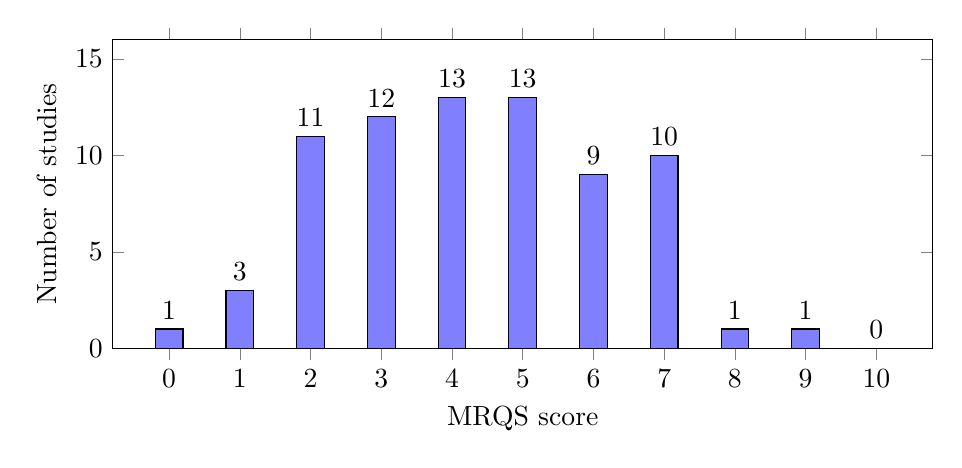
\begin{tikzpicture}
			\begin{axis}[
				width=12cm,
				height=5.5cm,
				ylabel={Number of studies},
				xlabel={MRQS score},
				xtick={0,1,2,3,4,5,6,7,8,9,10},
				ymin=0, ymax=16,
				ybar,
				bar width=10pt,
				nodes near coords,
				enlarge x limits=0.08,
				]
				\addplot[fill=blue!50] coordinates {
					(0,1) (1,3) (2,11) (3,12) (4,13) (5,13) (6,9) (7,10) (8,1) (9,1) (10,0)
				};
			\end{axis}
		\end{tikzpicture}
		\caption{Distribution of Methodological Reporting Quality Scores across 74 included studies.}
		\label{fig:mrqs_dist}
	\end{figure}
	
	The internal consistency of the MRQS was moderate (Cronbach's $\alpha$ = .58). This value is lower than the conventional threshold of .70 typically expected for psychometric scales, but is consistent with the intended design of the instrument: the ten items capture distinct dimensions of reporting quality (e.g., sampling, measurement, statistical reporting, conceptual clarity) rather than a single latent construct. Corrected item--total correlations ranged from \textit{r} = --0.13 (M10, limitations discussed) to \textit{r} = 0.50 (M7, inferential statistics). Items M6 (pre--post design), M7 (inferential statistics), and M3 (control group) showed the strongest associations with the total score (\textit{r}~=~0.48, 0.50, and 0.42, respectively), reflecting a quantitative-methods cluster. Items M8 (explicit definition, $r = 0.05$) and M9 (theoretical framework, $r = 0.11$) were largely independent of the remaining items, consistent with the observation that conceptual and theoretical practices do not co-vary with empirical design choices in this literature.
	
	\subsubsection{Item-level prevalence}
	\label{sec:results_rq2_items}
	
	Table~\ref{tab:mrqs_prevalence} presents the prevalence of each MRQS item, ordered from most to least commonly met. The items can be grouped into three tiers:
	
	\begin{table}[b]
		\centering
		\caption{MRQS item prevalence across 74 studies, with temporal comparison.}
		\label{tab:mrqs_prevalence}
		%\small
		\begin{tabular}{@{}clcccc@{}}
			\toprule
			\textbf{Item} & \hfill \textbf{Criterion} & \textbf{All (\textit{n}~=~74)} & \textbf{2004--17 (\textit{n}~=~37)} & \textbf{2018--24 (\textit{n}~=~37)} & \textbf{$\Delta$} \\
			\midrule
			M9 & Theoretical framework & 70 (94.6\%) & 34 (91.9\%) & 36 (97.3\%) & +5.4 \\
			M1 & Sample size reported & 62 (83.8\%) & 29 (78.4\%) & 33 (89.2\%) & +10.8 \\
			M2 & Sample $\geq 30$ & 37 (50.0\%) & 19 (51.4\%) & 18 (48.6\%) & $-2.7$ \\
			M10 & Limitations discussed & 35 (47.3\%) & 14 (37.8\%) & 21 (56.8\%) & +18.9 \\
			M6 & Pre--post design & 29 (39.2\%) & 16 (43.2\%) & 13 (35.1\%) & $-8.1$ \\
			M7 & Inferential statistics & 29 (39.2\%) & 14 (37.8\%) & 15 (40.5\%) & +2.7 \\
			M3 & Control group & 23 (31.1\%) & 14 (37.8\%) & 9 (24.3\%) & $-13.5$ \\
			M4 & Validated instruments & 16 (21.6\%) & 7 (18.9\%) & 9 (24.3\%) & +5.4 \\
			M8 & Explicit definition & 11 (14.9\%) & 7 (18.9\%) & 4 (10.8\%) & $-8.1$ \\
			M5 & Effect sizes reported & 7 (9.5\%) & 3 (8.1\%) & 4 (10.8\%) & +2.7 \\
			\bottomrule
		\end{tabular}
	\end{table}
	
	\begin{enumerate}
		\item 
		\textit{High-prevalence items (>75\%).} Two items were met by the large majority of studies. M9 (theoretical framework) was the most commonly met criterion (94.6\%), indicating that nearly all studies grounded their work in at least one named theoretical framework, though the depth and specificity of theoretical engagement varied considerably. M1 (sample size reported) was met by 83.8\% of studies, meaning that 12 studies (16.2\%) did not report participant numbers~-- typically design-description papers or prototype evaluations without formal empirical testing.
		
		\item 
		\textit{Mid-prevalence items (20--50\%).} Five items fell in the mid-range. M2 (sample $\geq 30$) was met by exactly half the studies. M10 (limitations discussed) was met by 47.3\%, showing a notable improvement from the earlier to the later period (+18.9 percentage points), suggesting that conventions around limitations reporting have strengthened over time. M6 (pre--post design) and M7 (inferential statistics) were each met by 39.2\%, and M3 (control group) by 31.1\%. The decline in control group usage from the earlier to the later period ($-$13.5 percentage points) is noteworthy and reflects the compositional shift toward qualitative and design-based studies in more recent years.
		
		\item 
		\textit{Low-prevalence items ($<$20\%).} Three items were met by fewer than one in five studies. M4 (validated instruments) was reported in only 21.6\% of studies, indicating that nearly four in five studies either used unvalidated measures, did not report instrument reliability, or relied on non-standardised assessment methods. M8 (explicit definition) was met by only 14.9\%, confirming the parent review's finding of pervasive definitional ambiguity. M5 (effect sizes) was the least commonly met criterion at 9.5\%, meaning that more than 90\% of studies~-- including those reporting inferential statistics~-- did not report standardised effect measures. This represents the single largest reporting gap in the corpus and severely limits the possibility of meta-analytic synthesis.
	\end{enumerate}
	
	%\paragraph{Temporal trends.} 
	The comparison between the earlier (2004--2017) and later (2018--2024) periods revealed a mixed pattern. Reporting of sample sizes (+10.8 pp), limitations (+18.9 pp), and validated instruments (+5.4 pp) improved over time. However, the use of control groups ($-$13.5 pp), pre--post designs ($-$8.1 pp), and explicit definitions ($-$8.1 pp) declined, suggesting that methodological sophistication in design has not accompanied improvements in reporting transparency.
	
	\subsubsection{MRQS by study-level characteristics}
	\label{sec:results_rq2_crosstab}
	
	Table~\ref{tab:mrqs_groups} presents the MRQS means by study-level grouping variables.
	
	\begin{table}[ht]
		\centering
		\caption{MRQS by study-level characteristics.}
		\label{tab:mrqs_groups}
		\small
		\begin{tabular}{@{}llccl@{}}
			\toprule
			\hfill \textbf{Variable} & \hfill \textbf{Group} & \textbf{\textit{n}} & \textbf{Mean (SD)} & \hfill \textbf{Test statistic} \\
			\midrule
			\multirow{3}{*}{Publication type} & Journal article & 24 & 4.75 (2.03) & \multirow{3}{*}{\textit{H} = 1.48, \textit{p} = .48} \\
			& Conference paper & 40 & 4.17 (1.80) & \\
			& Book chapter & 9 & 4.11 (2.09) & \\
			\addlinespace
			\multirow{3}{*}{Education level} & Primary & 10 & 4.80 (1.55) & \multirow{3}{*}{\textit{H} = 1.10, \textit{p} = .58} \\
			& Secondary & 35 & 4.46 (1.77) & \\
			& Higher education & 21 & 4.14 (2.41) & \\
			\addlinespace
			\multirow{2}{*}{Period} & 2004--2017 & 37 & 4.24 (2.17) & \multirow{2}{*}{\textit{U} = 657.5, \textit{p} = .77} \\
			& 2018--2024 & 37 & 4.38 (1.69) & \\
			\addlinespace
			\multirow{2}{*}{Explicit definition} & Present & 11 & 5.36 (1.69) & \multirow{2}{*}{\textit{U} = 467.0, \textit{p} = .065} \\
			& Absent & 63 & 4.13 (1.92) & \\
			\addlinespace
			\multirow{2}{*}{Overall ROB} & High & 62 & 4.13 (1.88) & \multirow{2}{*}{---} \\
			& Moderate or lower & 12 & 5.25 (1.86) & \\
			\bottomrule
		\end{tabular}
	\end{table}
	
	No statistically significant differences in MRQS were observed across publication types (Kruskal--Wallis \textit{H} = 1.48, \textit{p} = .48), education levels (\textit{H} = 1.10, \textit{p} = .58), or time periods (Mann--Whitney \textit{U} = 657.5, \textit{p} = .77). Journal articles scored slightly higher than conference papers (mean 4.75 vs.\ 4.17) and primary education studies scored slightly higher than higher education studies (4.80 vs.\ 4.14), but these differences were small and non-significant given the sample sizes involved.
	
	The comparison between studies with and without explicit gamification definitions approached but did not reach conventional significance (\textit{U} = 467.0, \textit{p} = .065). Studies providing explicit definitions scored higher on average (mean 5.36, SD = 1.69) than those that did not (mean 4.13, SD = 1.92), a difference of 1.23 points on the 10-point scale. While this difference cannot be interpreted as statistically robust given the small subgroup (\textit{n}~=~11), the direction is consistent with the hypothesis that definitional clarity is associated with more thorough reporting practices. This finding is examined further in section~\ref{sec:results_rq4}.
	
	Studies rated as having a high overall risk of bias scored lower on the MRQS (mean = 4.13, SD = 1.88) than those rated moderate or lower (mean = 5.25, SD = 1.86). The two studies rated ``Unclear'' for overall risk of bias were notable outliers, scoring 8 and 9 on the MRQS; these studies reported most methodological details but received ``Unclear'' domain ratings due to ambiguous signalling-question responses rather than identifiable flaws.
	
	\subsubsection{Inter-item relationships}
	\label{sec:results_rq2_interitem}
	
	Examination of inter-item associations revealed a quantitative-methods cluster: items M3 (control group), M6 (pre--post), and M7 (inferential statistics) were positively intercorrelated ($\phi_{M3 \times M6}$ = 0.48; $\phi_{M3 \times M7}$ = 0.36; $\phi_{M6 \times M7}$ = 0.60), indicating that studies employing one of these design features tended to employ the others. Items M1 and M2 (sample reporting and size) were also associated ($\phi$ = 0.44), as M2 is conditional on M1. In contrast, M8 (definition) and M9 (theoretical framework) were largely independent of the quantitative cluster, suggesting that the conceptual and empirical dimensions of methodological quality operate as separate factors in this literature.
	
	The near-zero item--total correlation for M8 (\textit{r} = 0.05) and the negative correlation for M10 (\textit{r} = --0.13) indicate that definitional clarity and limitations discussion, respectively, are orthogonal to the overall score and to each other. The negative direction of M10 is surprising and may reflect the fact that higher-scoring studies~-- which tend to employ experimental designs~-- less frequently discuss limitations than lower-scoring qualitative and design-based studies, where reflexive discussion of constraints is a disciplinary norm.
	
	
	% ===========================================================================
	% RESULTS — RQ3
	% ===========================================================================
	
	\subsection{RQ3: Risk-of-bias patterns}
	\label{sec:results_rq3}
	
	\subsubsection{Overall risk of bias}
	\label{sec:results_rq3_overall}
	
	Sixty-two of the 74 studies (83.8\%) were rated as having a high overall risk of bias. Nine studies (12.2\%) received a moderate rating, two (2.7\%) were rated unclear, and only one study (1.4\%) received a low overall rating. The single low-risk study \cite{15Slater2022} achieved low ratings on both Domain~2 (data collection and analysis) and Domain~3 (interpretation), with no domain rated high.
	
	Overall risk-of-bias ratings did not differ markedly between the earlier and later periods: 86\% of studies published in 2004--2017 were rated high, compared with 81\% of those published in 2018--2024. Journal articles had a somewhat lower proportion of high ratings (71\%) than conference papers (90\%) or book chapters (89\%), likely reflecting the longer format and more rigorous peer review associated with journal publication.
	
	\subsubsection{Domain-level analysis}
	\label{sec:results_rq3_domains}
	
	Domain-level risk-of-bias distributions revealed a clear gradient: Domain~1 (participant selection) was the weakest area, Domain~2 (data collection and analysis) was intermediate, and Domain~3 (interpretation and reporting) was the relative strength (figure~\ref{fig:rob_domains}).
	
	\begin{figure}[ht]
		\centering
		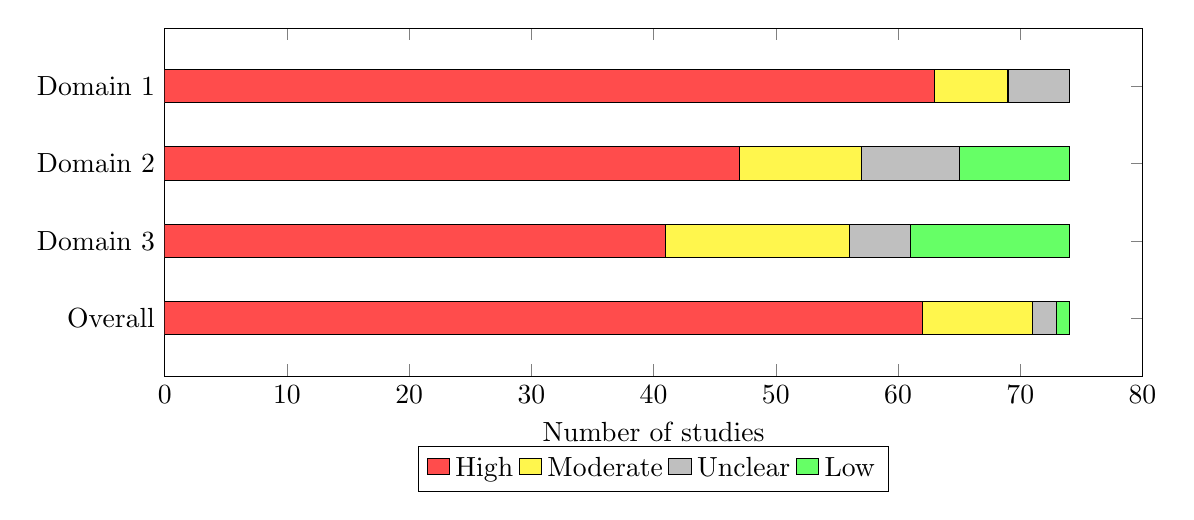
\begin{tikzpicture}
			\begin{axis}[
				width=14cm,
				height=6cm,
				xbar stacked,
				bar width=12pt,
				xlabel={Number of studies},
				symbolic y coords={Overall,Domain 3,Domain 2,Domain 1},
				ytick=data,
				legend style={at={(0.5,-0.2)}, anchor=north, legend columns=4},
				xmin=0, xmax=80,
				enlarge y limits=0.25,
				]
				\addplot[fill=red!70] coordinates {(62,Overall) (41,Domain 3) (47,Domain 2) (63,Domain 1)};
				\addplot[fill=yellow!70] coordinates {(9,Overall) (15,Domain 3) (10,Domain 2) (6,Domain 1)};
				\addplot[fill=gray!50] coordinates {(2,Overall) (5,Domain 3) (8,Domain 2) (5,Domain 1)};
				\addplot[fill=green!60] coordinates {(1,Overall) (13,Domain 3) (9,Domain 2) (0,Domain 1)};
				\legend{High, Moderate, Unclear, Low}
			\end{axis}
		\end{tikzpicture}
		\caption{Risk-of-bias ratings by domain and overall (\textit{n}~=~74). Domain~1: participant selection; Domain~2: data collection and analysis; Domain~3: interpretation and reporting.}
		\label{fig:rob_domains}
	\end{figure}
	
	\paragraph{Domain~1 (Participant selection and study context).} This was the most problematic domain, with 63 of 74 studies (85.1\%) rated high risk, six (8.1\%) moderate, five (6.8\%) unclear, and none achieving a low rating. Not a single study in the corpus received a favourable assessment of its sampling procedures across both signalling questions. The two constituent questions revealed why: Q1 (Are the criteria for selecting study participants clearly described?) received favourable responses for only 26 studies (35.1\%), while Q2 (Is the sample of participants representative of the target population?) received \emph{no} favourable responses across all 74 studies (0\%)~-- 55 studies (74.3\%) were rated unfavourable and 19 (25.7\%) were rated ambiguous. The universal failure on Q2 reflects the pervasive use of convenience samples, single-institution recruitment, and intact classroom groups throughout the literature.
	
	\paragraph{Domain~2 (Data collection and analysis).} Forty-seven studies (63.5\%) were rated high risk, ten (13.5\%) moderate, eight (10.8\%) unclear, and nine (12.2\%) low. Domain~2 showed the widest spread of ratings among the three domains, reflecting genuine variation in measurement practices. Q3 (Were valid and reliable tools used?) received favourable ratings for 16 studies (21.6\%) and unfavourable ratings for 35 (47.3\%), with 23 (31.1\%) rated ambiguous. Q4 (Are the methods of data analysis described and justified?) was favourable for 17 studies (23.0\%) and unfavourable for 39 (52.7\%). The nine studies receiving low risk on Domain~2 employed validated instruments with reported reliability coefficients and clearly described, justified analytic methods.
	
	\paragraph{Domain~3 (Interpretation and reporting).} This was the strongest domain relative to the other two, though 41 studies (55.4\%) were still rated high risk. Fifteen studies (20.3\%) received moderate ratings, five (6.8\%) unclear, and 13 (17.6\%) low~-- the highest proportion of low-risk ratings across any domain. Q5 (Are interpretations consistent with results?) was favourable for 25 studies (33.8\%) but drew the highest rate of ambiguous responses (41.9\%), reflecting the difficulty of assessing interpretive consistency from text alone. Q6 (Are limitations discussed?) was favourable for 35 studies (47.3\%), the highest favourable rate of any signalling question.
	
	\subsubsection{Domain co-occurrence profiles}
	\label{sec:results_rq3_profiles}
	
	The most common risk-of-bias profile was High--High--High across all three domains, characterising 32 of 74 studies (43.2\%). The next most frequent profiles each accounted for 3--5 studies: High--High--Moderate (\textit{n}~=~5), High--Moderate--Moderate (\textit{n}~=~4), Moderate--Moderate--Moderate (\textit{n}~=~3), and High--Low--Moderate (\textit{n}~=~3). In total, 18 studies (24.3\%) received a low rating in at least one domain, but in most cases, these low domain ratings were accompanied by high ratings in other domains, resulting in a high or moderate overall rating.
	
	The co-occurrence analysis revealed substantial overlap in domain-level weaknesses. Of the 63 studies rated high on Domain~1, 43 (68.3\%) were also rated high on Domain~2, and 37 (58.7\%) were also high on Domain~3. Thirty-two studies (43.2\%) were rated high across all three domains. This pattern suggests that methodological limitations are not confined to specific domains but tend to co-occur, reflecting a general lack of methodological rigour rather than domain-specific weaknesses.
	
	Notably, Domain~3 showed the greatest capacity for independent variation. Among the 63 studies rated high on Domain~1, 13 (20.6\%) achieved a low or moderate rating on Domain~3, indicating that some studies with weak sampling procedures nonetheless demonstrated sound interpretive practices. This asymmetry is pedagogically relevant: it suggests that sound interpretation and transparent reporting of limitations are achievable even within the practical constraints that make strong sampling procedures difficult in educational settings.
	
	\subsubsection{Risk of bias by study characteristics}
	\label{sec:results_rq3_crosstab}
	
	The proportion of studies rated high overall risk of bias was higher among conference papers (90\%, \textit{n}~=~36/40) than journal articles (71\%, \textit{n}~=~17/24). Higher education studies showed a marginally higher rate of high Domain~1 ratings (95\%, \textit{n}~=~20/21) than secondary education studies (77\%, \textit{n}~=~30/39), though this difference may partly reflect stricter sampling expectations applied to university-based research.
	
	Among the 11 studies providing explicit definitions of gamification, nine (81.8\%) were rated as having a high overall risk of bias, compared with 53 of 63 (84.1\%) among those without definitions. This negligible difference indicates that while definitional clarity is associated with slightly higher MRQS scores (as shown in section~\ref{sec:results_rq2}), it does not translate into lower risk-of-bias ratings, likely because the ROB assessment captures design features (sampling, measurement) that are largely independent of conceptual reporting practices.
	
	
	% ===========================================================================
	% RESULTS — RQ4 and RQ5
	% ===========================================================================
	
	\subsection{RQ4: Definitional practices and methodological quality}
	\label{sec:results_rq4}
	
	Only 11 of the 74 studies (14.9\%) provided explicit definitions of gamification, game-based learning, serious games, or related constructs. These 11 studies defined a range of constructs~-- gamification as the addition of game elements to non-game contexts \cite{43ali2018indonesian, 34Serrano2023}, serious games as applications not designed primarily for entertainment \cite{42Huffer201581, 41Petersen2023301}, digital game-based learning as a paradigm using games to convey educational content \cite{30Zin2008, 23Zin2009322}, and pervasive games as mobile experiences integrating physical and virtual environments \cite{58Shih2015173}. The terminological diversity among the definitional studies themselves underscores the absence of shared vocabulary.
	
	\subsubsection{Profile of definitional studies}
	
	Studies providing definitions were disproportionately published in journals (7 of 11, 63.6\%) compared with the overall corpus (24 of 74, 32.4\%), suggesting that the longer format and more detailed reporting expectations of journal articles may facilitate definitional clarity. Seven of the 11 definitional studies were published in 2004--2017, and only four in 2018--2024, indicating that definitional practices have not improved~-- and may have declined~-- over time. Studies with definitions cited more theoretical frameworks on average (mean = 5.55) than those without (mean = 4.11), suggesting a modest association between conceptual precision and theoretical grounding.
	
	\subsubsection{Association with methodological quality}
	
	As reported in section~\ref{sec:results_rq2}, studies providing explicit definitions scored higher on the MRQS (mean = 5.36, SD = 1.69) than those that did not (mean = 4.13, SD = 1.92), a difference of 1.23 points that approached but did not reach statistical significance (\textit{U} = 467.0, \textit{p} = .065). However, the two groups did not differ on overall risk-of-bias ratings: 81.8\% (9 of 11) of definitional studies and 84.1\% (53 of 63) of non-definitional studies were rated high risk.
	
	This divergence~-- higher MRQS but equivalent risk of bias~-- can be explained by the composition of the MRQS. Definitional studies gained an advantage over items relating to reporting transparency (M1, M8, M9, M10) rather than over items relating to study design (M3, M6, M7). The risk-of-bias assessment, by contrast, is heavily influenced by design features (sampling, measurement validity) on which definitional studies showed no advantage. The implication is that definitional clarity functions as a marker of reporting conscientiousness rather than as a driver of stronger study design.
	
	\subsection{RQ5: LLM validation}
	\label{sec:results_rq5}
	
	\subsubsection{Risk-of-bias assessment: GPT-4o vs.\ verified judgments}
	\label{sec:results_rq5_rob}
	
	Comparison of GPT-4o's original signalling-question responses (from the extraction spreadsheet) against the final verified responses (from the JSON records) revealed substantial modification during human verification. Overall percentage agreement across all six signalling questions and all 74 studies was 37.6\% (167 of 444 question--study pairs).
	
	Table~\ref{tab:llm_rob_agreement} presents the question-level agreement rates. Q6 (limitations discussed) had the highest agreement (52.7\%), while Q3 (validated instruments) had the lowest (29.7\%). Cohen's $\kappa$ was computed for question--study pairs where both the GPT-4o and verified responses used the standard three-level scheme (yes/no/unclear), yielding values ranging from $\kappa$ = --0.04 (Q3) to $\kappa$ = 0.21 (Q6). By the benchmarks of \citet{LandisKoch1977}, five of six questions showed only slight agreement ($\kappa$ < 0.20), and Q6 showed fair agreement.
	
	\begin{table}[ht]
		\centering
		\caption{Agreement between GPT-4o and final verified risk-of-bias signalling question responses (\textit{n}~=~74 studies).}
		\label{tab:llm_rob_agreement}
		%\small
		\begin{tabular}{@{}lccc@{}}
			\toprule
			\hfill \textbf{Question} & \textbf{Domain} & \textbf{Agreement (\%)} & \textbf{$\kappa$\textsuperscript{a}} \\
			\midrule
			Q1: Selection criteria described & D1 & 39.2 & 0.02 \\
			Q2: Sample representative & D1 & 35.1 & $-0.01$ \\
			Q3: Validated instruments & D2 & 29.7 & $-0.04$ \\
			Q4: Analysis methods justified & D2 & 36.5 & 0.08 \\
			Q5: Interpretation consistent & D3 & 32.4 & $-0.02$ \\
			Q6: Limitations discussed & D3 & 52.7 & 0.21 \\
			\midrule
			\textbf{Overall} & & \textbf{37.6} & ~--  \\
			\bottomrule
			\multicolumn{4}{@{}l@{}}{\textsuperscript{a}~Computed on subset where both raters used standard yes/no/unclear responses.}
		\end{tabular}
	\end{table}
	
	The dominant pattern of disagreement was a shift from more favourable GPT-4o ratings to less favourable verified ratings. For Q2 (sample representativeness), GPT-4o judged 33 studies as ``unclear'' that were verified as ``no'', and a further five originally rated ``yes'' were changed to ``no''. For Q4 (analysis methods), 21 GPT-4o ``yes'' responses were changed to ``no'' during verification, and nine were changed to ``moderate concern''. This pattern suggests that GPT-4o consistently applied less stringent criteria when assessing methodological features, a finding consistent with the parent review's observation that Claude~3.5~Sonnet and Claude~3~Haiku performed better than GPT-4o on risk-of-bias tasks.
	
	A complicating factor is that the final verified responses used a wider range of categories (including ``moderate concern'', ``some concerns'', ``partial'', and ``low concern'') than the three-level scheme (yes/no/unclear) specified in the GPT-4o prompt. This response-format mismatch inflates the measured disagreement rate, because many instances of ``disagreement'' reflect recoding into new categories rather than substantive reversal of judgments. For example, across all six questions, 62 of the 277 disagreements (22.4\%) involved a change from a standard GPT-4o response to a ``moderate'' or ``some concerns'' category not available to GPT-4o.
	
	\subsubsection{Data extraction consistency across LLMs}
	\label{sec:results_rq5_extraction}
	
	A supplementary dataset provided independent data extractions from three additional LLMs (Gemini~3~Pro, ChatGPT-4, and Grok~4.1-thinking) across all 80 candidate studies using the same 21-item prompt. Pairwise agreement was computed on two objective fields: publication year and publication type.
	
	For publication year, agreement rates ranged from 82.4\% (Gemini vs.\ ChatGPT-4) to 97.1\% (Gemini vs.\ Grok). Grok and Gemini showed the highest concordance, while ChatGPT-4 showed the most disagreement with both other models, producing year values that differed from the other two for approximately 14--18\% of studies. Year extraction was non-trivial for several studies in the corpus~-- particularly older conference papers that did not display the publication year on the first page or embedded it only in copyright notices~-- which explains some of the disagreement.
	
	For publication type (normalised to journal article, conference paper, book chapter), agreement ranged from 81.0\% (Gemini vs.\ ChatGPT-4) to 94.9\% (Gemini vs.\ Grok). Disagreements typically involved the classification of papers published in edited volumes or conference-affiliated special issues, where the boundary between ``conference paper'' and ``book chapter'' is genuinely ambiguous.
	
	These results suggest that LLM extraction of simple factual metadata achieves moderate to high agreement (approximately 80--97\% depending on the pair and the field), with agreement highest for unambiguous fields (year) and lower for fields requiring classificatory judgement (publication type). The substantially lower agreement observed for risk-of-bias signalling questions (37.6\%) likely reflects both the greater subjectivity of those judgements and the response-format mismatch noted above.
	
	\subsubsection{Implications for LLM-assisted research synthesis}
	
	The LLM validation findings point to a domain-specificity in LLM reliability: factual extraction (metadata, sample sizes, study design labels) can achieve acceptable agreement, but evaluative judgements (risk of bias, instrument validity, interpretive consistency) show agreement rates that are near chance levels without human oversight. This finding has implications for the trustworthiness of the parent review's data and, more broadly, for the growing use of LLMs in systematic review processes. Specifically, it suggests that LLM-assisted extraction can be a useful first-pass tool for factual metadata but should not be treated as a substitute for human assessment on evaluative dimensions.
	
	
	% ===========================================================================
	% SECTION 4: DISCUSSION
	% ===========================================================================
	
	\section{Discussion}
	\label{sec:discussion}
	
	This study examined the methodological quality and reporting practices of 74 studies on gamification in history education, drawn from a prior systematic review \cite{KorniienkoSemerikov2024}. The findings reveal a field characterised by widespread methodological limitations, a mean Methodological Reporting Quality Score of 4.31 out of 10, high risk of bias in 83.8\% of studies, and near-complete absence of effect size reporting and validated measurement instruments. This section interprets these findings, situates them within broader methodological discourse, discusses the implications of the LLM validation results, acknowledges limitations, and proposes directions for future research.
	
	\subsection{Summary and interpretation of principal findings}
	\label{sec:discussion_summary}
	
	The MRQS analysis revealed a three-tiered structure of reporting practices. Nearly universal compliance was observed on two items: theoretical frameworks (94.6\%) and sample size reporting (83.8\%). In contrast, a cluster of mid-range items~-- pre--post designs, inferential statistics, control groups, and limitations discussion~-- were each met by roughly 30--50\% of studies. The bottom tier~-- effect sizes (9.5\%), explicit definitions (14.9\%), and validated instruments (21.6\%)~-- exposes the most consequential reporting gaps.
	
	The near-total absence of effect size reporting (9.5\%) is perhaps the single most significant finding for the field's evidence base. Without standardised effect measures, meta-analytic synthesis is impossible, cross-study comparison is severely constrained, and the practical magnitude of gamification's impact on learning outcomes remains unknown. This problem is not unique to gamification research~-- effect size underreporting has been documented across educational technology and social science literatures \cite{Clark2016}~-- but its prevalence here is particularly troubling given the optimistic tone that characterises much of the primary literature.
	
	The risk-of-bias analysis complemented the MRQS by identifying a clear gradient across the three assessed domains. Domain~1 (participant selection) was universally problematic: not a single study received a favourable rating on sample representativeness (Q2). This result reflects the near-universal reliance on convenience samples~-- intact classrooms, volunteer participants, and single-institution recruitment~-- which is understandable given the practical constraints of educational research but fundamentally limits the external validity of the findings. Domain~3 (interpretation) showed the greatest relative strength, with 17.6\% of studies achieving a low-risk rating, suggesting that sound interpretive practices are achievable even in studies that are otherwise limited. The observation that 43.2\% of studies were rated high risk across all three domains simultaneously indicates that methodological weaknesses tend to co-occur rather than being localised.
	
	\subsection{Comparison with prior methodological assessments}
	\label{sec:discussion_comparison}
	
	The methodological limitations documented here are broadly consistent with concerns raised in prior reviews of gamification research. \citet{DichevDicheva2017} noted the prevalence of small samples, lack of control groups, and inconsistent operationalisation of gamification in their review of gamification in education, observing that the evidence for gamification's effectiveness was ``not very convincing'' when methodological quality was considered. \citet{KoivistoHamari2019} similarly reported that a majority of reviewed gamification studies lacked rigorous experimental designs. The mean MRQS of 4.31 provides a quantitative benchmark that gives precision to these qualitative observations: the typical study in this literature meets fewer than half of the ten basic methodological reporting criteria.
	
	How does the gamification-in-history-education literature compare with adjacent fields? The use of different quality instruments complicates direct numerical comparison, but several reference points are informative. \citet{Connolly2012} reviewed 129 empirical studies of game-based learning and noted that only 14\% employed experimental or quasi-experimental designs with control groups~-- comparable to the 31.1\% observed here. The higher rate in the present corpus may partly reflect the stricter inclusion criteria of the parent review, which excluded non-empirical studies. \citet{Clark2016} found that effect sizes were reported in only a minority of game-based learning studies, consistent with the 9.5\% rate documented here. These comparisons suggest that the gamification-in-history-education literature is neither substantially better nor worse than the broader educational gaming literature in its methodological practices, but rather reflects a field-wide norm of underreporting.
	
	The temporal analysis yielded a nuanced picture: some reporting practices have improved over time (sample size disclosure, limitations discussion), while others have declined (control group usage, explicit definitions). This divergence suggests that the field's growth since 2018 has been driven primarily by qualitative, design-based, and descriptive studies that expand the literature's topical and methodological diversity but do not strengthen its inferential foundations. The field is not uniformly improving; it is diversifying.
	
	\subsection{The definitional gap}
	\label{sec:discussion_definitions}
	
	The finding that only 14.9\% of studies provided an explicit definition of gamification, game-based learning, or a related construct warrants particular attention. This rate is lower than the definitional provision rates reported in broader gamification reviews~-- \citet{KoivistoHamari2019} found that the majority of studies in their corpus referenced \citeauthor{Deterding2011}'s \cite{Deterding2011} definition, though many did so uncritically. The lower rate observed here may reflect the disciplinary composition of the corpus: many studies were authored by historians, educators, or computer scientists rather than gamification researchers, and these authors may view the concept as self-evident rather than as requiring formal definition.
	
	The modest association between definitional clarity and higher MRQS scores (5.36 vs.\ 4.13, \textit{p} = .065) suggests that definitional provision functions as a marker of general reporting conscientiousness rather than as a driver of stronger study design. Studies that take the time to define their central construct also tend to report sample sizes, discuss limitations, and cite theoretical frameworks more consistently. However, definitional provision was not associated with lower risk-of-bias ratings, indicating that construct clarity is necessary but not sufficient for methodological rigour.
	
	\subsection{Implications for evidence synthesis}
	\label{sec:discussion_synthesis}
	
	The combination of small samples (median \textit{n}~=~33.5), rare reporting of effect sizes (9.5\%), limited use of control groups (31.1\%), and a high risk of bias (83.8\%) has direct consequences for the strength of the evidence base. Meta-analytic pooling~-- the standard tool for quantitative synthesis~-- is effectively foreclosed by the absence of effect sizes, the heterogeneity of outcome measures, and the variability of study designs. Even narrative synthesis is complicated by the difficulty of comparing studies that use different definitions, measure different outcomes, and employ different populations.
	
	The implication for practice is that claims about the effectiveness of gamification in history education rest on a fragile evidentiary foundation. This is not to say that gamification is ineffective~-- several individual studies report substantial learning gains~-- but that the field-level evidence does not yet permit confident generalisation about \emph{when}, \emph{how}, and \emph{for whom} gamification works. Practitioners considering gamification adoption should approach the literature with appropriate caution, attend to the methodological quality of individual studies, and recognise that positive findings from studies with a high risk of bias may not replicate in different contexts.
	
	\subsection{LLM reliability: implications and limitations}
	\label{sec:discussion_llm}
	
	The LLM validation analysis revealed striking domain-specific reliability. Factual metadata extraction (publication year, publication type) achieved moderate to high agreement across models (82--97\%), while risk-of-bias signalling questions showed near-chance agreement between GPT-4o and the final verified assessments (37.6\% overall, $\kappa$ = --0.04 to 0.21). This pattern is consistent with emerging evidence in the broader LLM-for-systematic-reviews literature. \citet{Taneri2025} reported that ChatGPT-4o achieved moderate agreement ($\kappa$ = 0.51) with human reviewers on RoB~2 overall judgments in Cochrane Reviews, while \citet{Rubinstein2025} found that GPT-4 performed well at recommending articles for exclusion during screening but less well at inclusion decisions. \citet{MalekiKarami2024} cautioned that the subjectivity inherent in risk-of-bias assessment makes it particularly ill-suited for unsupervised AI applications.
	
	The low agreement observed in the present study is partly attributable to a response-format mismatch: GPT-4o was prompted to respond with yes/no/unclear, while the final verified assessments introduced additional categories (moderate concern, some concerns, partial) that were not available to GPT-4o. This inflation of measured disagreement is a methodological artefact rather than a substantive finding, but it does illustrate a practical challenge in LLM validation~-- namely, that post-hoc human modification of LLM outputs confounds the measurement of initial agreement.
	
	More substantively, the dominant pattern of disagreement was a shift from more favourable GPT-4o ratings to less favourable verified ratings, particularly on Q2 (sample representativeness) and Q4 (analysis methods). This suggests that GPT-4o applied less stringent evaluative criteria than human reviewers~-- a form of ``leniency bias'' that has been observed in other LLM evaluation contexts. For systematic review teams considering LLM-assisted risk-of-bias assessment, this finding reinforces the importance of human verification as a non-optional safeguard rather than a supplementary check.
	
	\subsection{Limitations of this study}
	\label{sec:discussion_limitations}
	
	Several limitations should be acknowledged.
	
	First, the MRQS is a purpose-built instrument that has not been externally validated. Its moderate internal consistency ($\alpha$ = .58) reflects the heterogeneity of the ten constituent items, which span sampling, measurement, statistical reporting, and conceptual clarity. The instrument functions as a reporting checklist rather than as a psychometric scale measuring a unitary construct, and its scores should be interpreted as summary descriptors of reporting completeness rather than as precise measures of methodological quality. Two items in particular~-- M8 (definition) and M10 (limitations)~-- showed near-zero or negative item--total correlations, suggesting that they operate independently of the empirical design cluster and might be more informative as standalone indicators.
	
	Second, the MRQS is biased toward quantitative research designs. Studies employing qualitative, case study, or design-based research methodologies will systematically score lower because several items (M2, M3, M5, M6, M7) are not applicable to these designs. The mean MRQS should therefore not be interpreted as implying that qualitative studies are inherently inferior; instead, the instrument measures the presence of quantitative reporting features. A complementary quality instrument tailored to qualitative designs would be needed for a more equitable cross-design comparison.
	
	Third, all analyses operate on data extracted by GPT-4o and verified by a single researcher in the parent review. The LLM validation analysis (section~\ref{sec:results_rq5}) demonstrates that GPT-4o's assessments were substantially modified during verification, particularly for evaluative judgments. While this verification process is expected to have improved the data, it also means that the final dataset reflects one researcher's post-hoc judgments applied to LLM-generated first drafts, introducing an unquantified degree of single-rater subjectivity.
	
	Fourth, no original study PDFs were re-examined for this analysis. All MRQS and risk-of-bias computations rely on the structured data fields in the JSON extraction records. If a study reported effect sizes, validated instruments, or other relevant details in sections of the paper not captured by the 21-item extraction prompt, this information would not be reflected in our analysis. The MRQS item prevalence rates should therefore be interpreted as lower bounds on actual reporting rates.
	
	Fifth, the ``Moderate'' risk-of-bias category present in the data deviates from the three-level scheme (Low/High/Unclear) specified in the adapted ROBIS protocol. Its introduction during human verification introduces a protocol deviation whose effects on the distribution of overall ratings are difficult to quantify.
	
	Sixth, this study is a secondary analysis of a single systematic review. The 74 studies represent the complete set of included studies rather than a probability sample, meaning that inferential statistics serve a descriptive rather than a confirmatory function. The generalisability of these findings is limited to the specific literature on gamification in history education identified by the parent review's search strategy.
	
	\subsection{Recommendations for future research}
	\label{sec:discussion_recommendations}
	
	The findings suggest five priorities for strengthening the evidence base:
	
	\begin{enumerate}
		\item 
		
		\textit{Report effect sizes.} The most impactful single improvement would be the routine reporting of standardised effect sizes (Cohen's $d$, $\eta^2$, or similar) alongside inferential statistics. This practice, already required by many psychology and education journals, would enable future meta-analytic synthesis and transform the evidence base from a collection of individual narratives into a cumulatively informative body of knowledge.
		
		\item 
		
		\textit{Use comparison groups.} Studies aiming to evaluate the effectiveness of gamification interventions should include comparison conditions, even if full randomisation is impractical. Waitlist controls, matched comparison groups, or alternating treatment designs can all strengthen causal inference relative to single-group pretest--posttest designs.
		
		\item 
		
		\textit{Define the construct.} Authors should explicitly state which construct they are investigating~-- gamification, game-based learning, serious games, or another variant~-- and provide a definition with specific enough boundaries to distinguish the intervention from related approaches. Where the study uses an established definition (e.g., \citet{Deterding2011}), this should be cited; where a novel conceptualisation is employed, its boundaries should be articulated.
		
		\item 
		
		\textit{Validate instruments.} Where quantitative outcomes are measured, instruments should be drawn from the validated literature where possible, or their psychometric properties (internal consistency, test--retest reliability, content validity) should be reported. The near-absence of instrument validation in the current corpus (21.6\%) represents a fundamental threat to measurement validity.
		
		\item 
		
		\textit{Pre-register studies and protocols.} Pre-registration of hypotheses, analysis plans, and outcome measures would reduce the risk of selective reporting and post-hoc hypothesis generation that inflates false-positive rates in small-sample studies. For systematic reviews in this domain, prospective protocol registration in PROSPERO or a similar registry should become standard practice.
	\end{enumerate}
	
	\subsection{Recommendations for LLM-assisted systematic reviews}
	\label{sec:discussion_llm_recs}
	
	The LLM validation findings suggest several practical guidelines for review teams:
	
	\begin{enumerate}%[noitemsep]
		\item Use LLMs for factual metadata extraction (year, country, sample size, publication type), where agreement rates are high, and errors are easily detected during quality checks.
		\item Do not use LLMs as unsupervised assessors for evaluative judgments (risk of bias, instrument validity, interpretive quality). Human verification should be mandatory for these tasks.
		\item When comparing LLM outputs to human verification, ensure that both raters use the same response format~-- introducing new categories during verification confounds agreement measurement.
		\item Report LLM agreement statistics (percentage agreement, $\kappa$) alongside substantive findings, so that readers can calibrate their confidence in the data.
		\item When multiple LLMs are used, compute pairwise agreement to identify items where model outputs diverge, as these items likely require closer human scrutiny.
	\end{enumerate}
	
	
	% ===========================================================================
	% SECTION 5: CONCLUSION
	% ===========================================================================
	
	\section{Conclusion}
	\label{sec:conclusion}
	
	This study provides the first systematic quantification of methodological quality and reporting practices in the gamification-in-history-education literature, examining 74 studies from a prior systematic review through a purpose-built Methodological Reporting Quality Score and a domain-level risk-of-bias re-analysis.
	
	Pervasive methodological limitations characterise the evidence base. The mean MRQS score of 4.31 out of 10 indicates that the typical study meets fewer than half of the 10 basic reporting criteria. Effect sizes are reported in only 9.5\% of studies, validated measurement instruments in 21.6\%, and explicit definitions of gamification in 14.9\%. A high risk of bias was identified in 83.8\% of studies, with participant selection procedures universally inadequate (0\% favourable for sample representativeness). These findings do not invalidate the predominantly positive effectiveness claims in the literature, but they do indicate that these claims rest on a narrow evidential foundation that limits confident generalisation.
	
	Three findings merit particular emphasis. First, methodological quality has not improved commensurately with the growth of the field: while reporting transparency has increased since 2018 (more studies report sample sizes and discuss limitations), the adoption of stronger research designs (control groups, pre--post measurement) has declined, reflecting a compositional shift toward qualitative and design-based studies. Second, definitional clarity functions as a marker of reporting conscientiousness rather than a determinant of design quality~-- studies that define their central construct report more completely but do not design their studies more rigorously. Third, LLM-assisted risk-of-bias assessment showed near-chance agreement with human-verified judgments ($\kappa$ = --0.04 to 0.21), demonstrating that automated evaluative assessment requires mandatory human oversight, even as factual metadata extraction achieves acceptable reliability (82--97\% agreement).
	
	The MRQS instrument and the domain-level risk-of-bias analysis developed here are replicable and transferable. We encourage their application in adjacent fields~-- such as gamification in STEM education, game-based language acquisition, or educational technology interventions more broadly~-- to enable cross-domain comparisons of methodological maturity. In the field of gamification in history education specifically, the most impactful improvements would be routine reporting of effect sizes, the use of comparison groups, and the validation of measurement instruments. These changes would transform the evidence base from one that supports optimistic narratives to one that enables rigorous synthesis.
	
	\begin{dataavailability}
		All structured data files, extraction records, and analysis scripts underlying this study are available at \url{https://tinyurl.com/msw66d6k}.
	\end{dataavailability}
	
	\begin{authorcontributions}
		Conceptualisation, resources, supervision, and validation, Serhiy O. Semerikov; data curation, formal analysis, and investigation, Serhii S. Korniienko; methodology, software, visualisation, writing -- original draft, and writing -- review and editing, Serhii S. Korniienko and Serhiy O. Semerikov. All authors have read and agreed to the published version of the manuscript.
	\end{authorcontributions}
	
	\begin{conflictsofinterest}
		The authors declare no conflict of interest.
	\end{conflictsofinterest}
	
	%\begin{acknowledgments}
	%The authors thank the developers of the open-source tools used in this analysis, including Python, \texttt{scipy}, and \texttt{pandas}. The large language models GPT-4o (OpenAI), Claude 3.5 Sonnet (Anthropic), Gemini 3 Pro (Google), and Grok 4.1-thinking (xAI) were used for data extraction tasks as documented in the Methods section.
	%\end{acknowledgments}
	
	\begin{aideclaration}
		Large language models were used at multiple stages of this research. In the parent systematic review \cite{KorniienkoSemerikov2024}, GPT-4o (OpenAI) was used for structured data extraction and an initial risk-of-bias assessment; Claude~3.5~Sonnet (Anthropic) for eligibility screening; and Claude~3~Opus and Claude~3~Haiku (Anthropic) for comparative risk-of-bias evaluation. In the supplementary multi-LLM comparison reported in section~\ref{sec:results_rq5_extraction}, Gemini~3~Pro (Google), ChatGPT-4 (OpenAI), and Grok~4.1-thinking (xAI) independently performed data extraction using the same structured prompt. All LLM outputs used in the parent review were verified and, where necessary, corrected by human researchers, as documented in the Methods section. For the preparation of this manuscript, Claude Opus~4.6 (Anthropic) was used via Claude Code as a writing and coding assistant to support drafting, statistical analysis scripting in Python, and iterative revision of the manuscript text. The authors assume full responsibility for the accuracy, integrity, and originality of all content. All AI-generated outputs were critically reviewed, verified, and substantively edited by the authors prior to submission.
	\end{aideclaration}
	
	%\bibliographystyle{cas-model2-names}
	\bibliography{references}
	
\end{document}
